% Vietnamese translation for OI Public Library
% Source-File: IOI中国国家候选队论文/2005/蒋炎岩/蒋炎岩.ppt
\documentclass[11pt]{article}
\usepackage{oipl-vn}
\usepackage{tikz}
\usetikzlibrary{arrows.meta,positioning}

\newcommand{\Oh}{\mathcal{O}}

\title{Bản trình chiếu: Treap}
\author{Jiang Yanyan}
\date{2005}

\begin{document}
\maketitle

\origtitle{Treap: bản trình chiếu}
\sourcepath{IOI China candidate team papers / 2005 / Jiang Yanyan / Jiang Yanyan.ppt}

\section{Mạch trình bày}

Tệp gốc chỉ có PowerPoint và phần lớn nội dung là hiệu ứng/hình vẽ. Văn bản
trích xuất được từ slide xác nhận các mốc: \textit{Treap},
\(\Oh(\log n)\), \(\sqrt n\), \(2\sqrt n\), \textit{Dynamic Ranking},
\textit{Replace Element} và trang kết thúc. Vì vậy bản ghi chú này phục hồi
mạch chắc chắn nhất của bản trình chiếu: giới thiệu treap như cây cân bằng
ngẫu nhiên, sau đó liên hệ tới truy vấn xếp hạng động và thao tác thay phần
tử. Những đoạn hình minh họa trong PPT không đọc được ổn định, nên bản dịch
phục dựng các sơ đồ cốt lõi: bất biến treap và thao tác tách/gộp.

\section{Treap là gì}

Treap kết hợp cây tìm kiếm nhị phân theo khóa với heap theo độ ưu tiên ngẫu
nhiên. Mỗi nút có một khóa để giữ thứ tự inorder, và một độ ưu tiên để giữ
tính cân bằng kỳ vọng. Nếu gọi khóa là \(key\) và độ ưu tiên là \(prio\), cây
phải thỏa đồng thời:
\[
  key(\text{con trái}) < key(\text{gốc}) < key(\text{con phải}),
\]
và \(prio\) của gốc tốt hơn \(prio\) của các con theo quy ước heap.

Có hai cách nhìn tương đương. Cách thứ nhất là chèn khóa như cây tìm kiếm nhị
phân, rồi quay nút mới lên cho tới khi thứ tự heap theo độ ưu tiên được khôi
phục. Cách thứ hai là xem các độ ưu tiên ngẫu nhiên quyết định hình dạng cây:
trong một tập khóa, nút có độ ưu tiên tốt nhất làm gốc, phần khóa nhỏ hơn nằm
bên trái, phần khóa lớn hơn nằm bên phải. Vì độ ưu tiên là hoán vị ngẫu
nhiên, chiều cao kỳ vọng là \(\Oh(\log n)\), dẫn tới mốc \(\Oh(\log n)\) còn
đọc được trong slide.

\begin{figure}[ht]
\centering
\begin{tikzpicture}[
  v/.style={circle, draw, minimum size=8mm, inner sep=0pt, align=center},
  edge/.style={-Latex},
  level distance=1.1cm,
  sibling distance=2.1cm
]
\node[v] {40\\\(p=3\)}
  child {node[v] {20\\\(p=7\)}
    child {node[v] {10\\\(p=9\)}}
    child {node[v] {30\\\(p=8\)}}}
  child {node[v] {70\\\(p=5\)}
    child {node[v] {60\\\(p=6\)}}
    child {node[v] {90\\\(p=10\)}}};
\node[below=4.0cm, align=center]
  {Khóa tăng theo inorder; độ ưu tiên nhỏ hơn nằm cao hơn theo quy ước heap.};
\end{tikzpicture}
\caption{Một treap đồng thời là cây tìm kiếm nhị phân theo khóa và heap theo độ ưu tiên.}
\end{figure}

\section{Thao tác cơ bản}

Tìm kiếm trong treap giống hệt cây tìm kiếm nhị phân. Chèn một nút gồm hai
bước: đi theo khóa để đặt nút vào vị trí lá, rồi dùng các phép quay trái/phải
để sửa tính chất heap. Xóa một nút cũng có thể làm bằng quay nút đó xuống dưới
cho tới khi thành lá, hoặc bằng tách và gộp hai cây con của nó.

Một cách cài hiện đại hơn dùng hai thao tác \(\operatorname{split}\) và
\(\operatorname{merge}\). \(\operatorname{split}(T,x)\) tách cây thành hai
cây chứa các khóa \(\le x\) và \(>x\). \(\operatorname{merge}(A,B)\) gộp hai
cây khi mọi khóa trong \(A\) nhỏ hơn mọi khóa trong \(B\), chọn gốc theo độ ưu
tiên rồi đệ quy vào một phía. Từ hai thao tác này có thể xây dựng chèn, xóa,
tìm hạng, tìm phần tử hạng \(k\) và xử lý dãy. Bản ghi chú chỉ nêu ý tưởng vì
mã nguồn hoàn chỉnh của treap khá dài và không phải phần chữ trích được từ
slide.

\begin{figure}[ht]
\centering
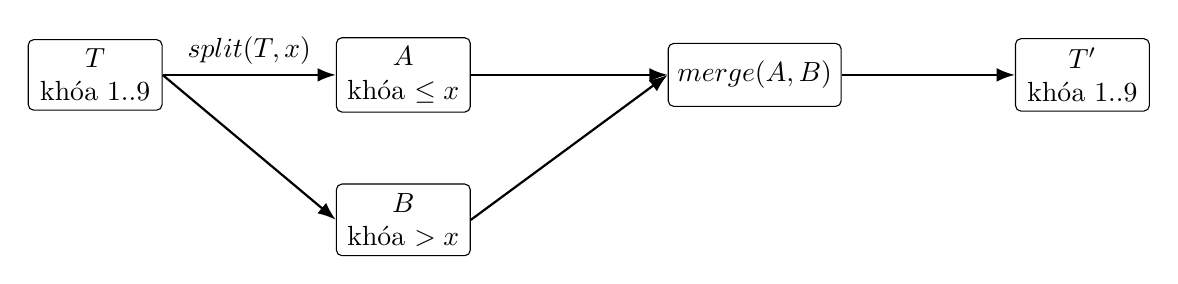
\begin{tikzpicture}[
  box/.style={draw, rounded corners=2pt, minimum width=1.7cm, minimum height=0.8cm, align=center},
  arrow/.style={-Latex, thick},
  node distance=1.2cm
]
\node[box] (t) {\(T\)\\khóa \(1..9\)};
\node[box, right=2.2cm of t] (a) {\(A\)\\khóa \(\le x\)};
\node[box, below=0.9cm of a] (b) {\(B\)\\khóa \(>x\)};
\draw[arrow] (t.east) -- node[above] {\(\operatorname{split}(T,x)\)} (a.west);
\draw[arrow] (t.east) -- (b.west);

\node[box, right=2.5cm of a] (m) {\(\operatorname{merge}(A,B)\)};
\node[box, right=2.2cm of m] (u) {\(T'\)\\khóa \(1..9\)};
\draw[arrow] (a.east) -- (m.west);
\draw[arrow] (b.east) -- (m.west);
\draw[arrow] (m.east) -- (u.west);
\end{tikzpicture}
\caption{Hai thao tác nền của treap hiện đại: tách theo khóa rồi gộp hai cây có miền khóa rời nhau.}
\end{figure}

\section{Vì sao hữu ích}

Trong lập trình thi đấu, treap thường được dùng khi cần một cây cân bằng dễ
cài đặt, hỗ trợ thao tác theo thứ tự, thống kê thứ hạng, hoặc xử lý dãy bằng
implicit treap. So với một số cây cân bằng chặt chẽ hơn, treap đơn giản và
linh hoạt.

\section{Xếp hạng động}

Slide có nhãn \textit{Dynamic Ranking}, nên ví dụ nhiều khả năng là bài toán
duy trì một tập hoặc một dãy có cập nhật và truy vấn hạng. Với treap theo
khóa, mỗi nút lưu thêm kích thước cây con. Khi đi tìm hạng của khóa \(x\), ta
đếm số phần tử nhỏ hơn \(x\) bằng kích thước các cây con trái đã bỏ qua. Khi
tìm phần tử hạng \(k\), ta so sánh \(k\) với kích thước cây con trái của nút
hiện tại để quyết định đi trái, trả về gốc hay đi phải.

Nếu dữ liệu cho phép nhiều khóa bằng nhau, có thể thêm trường số lần xuất hiện
ở mỗi nút, hoặc tách khóa thành cặp gồm giá trị và mã định danh. Khi đó xóa
một bản sao và chèn một bản sao đều vẫn có độ phức tạp kỳ vọng
\(\Oh(\log n)\). Đây là lý do treap hay được dùng trong bài có thao tác
``thay phần tử'': xóa giá trị cũ khỏi cấu trúc thứ tự, chèn giá trị mới, rồi
cập nhật mảng gốc.

\section{Thay phần tử và phân khối}

Các mốc \(\sqrt n\) và \(2\sqrt n\) trong PPT gợi ý phần minh họa về phân
khối cho bài xếp hạng động trên dãy. Một cách rất phổ biến là chia dãy thành
các khối kích thước khoảng \(\sqrt n\). Mỗi khối lưu các phần tử của nó trong
một cấu trúc có thứ tự, chẳng hạn mảng sắp xếp hoặc treap. Truy vấn trên đoạn
\([l,r]\) được tách thành các khối nguyên nằm giữa và hai phần thừa ở biên.
Với các khối nguyên, ta đếm nhanh số phần tử không vượt quá \(w\); với phần
biên, duyệt trực tiếp. Vì số khối và kích thước biên đều khoảng \(\sqrt n\),
biểu thức \(\sqrt n\) và \(2\sqrt n\) xuất hiện tự nhiên trong phân tích.

Thao tác \textit{Replace Element} tương ứng với thay \(A[i]\) bằng giá trị
mới. Trong phân khối, chỉ khối chứa \(i\) bị ảnh hưởng: xóa giá trị cũ khỏi
cấu trúc của khối, chèn giá trị mới, rồi sửa mảng. Nếu cấu trúc trong khối là
mảng sắp xếp, cập nhật có thể tốn tuyến tính theo kích thước khối. Nếu dùng
treap, cập nhật trong khối là \(\Oh(\log n)\) kỳ vọng, đổi lại mã phức tạp
hơn. Với truy vấn hạng \(k\) trên đoạn, ta vẫn thường dùng hàm đếm theo
ngưỡng rồi nhị phân giá trị, giống tư tưởng của bài \textit{Dynamic Rankings}.

\section{Treap ẩn}

Một nhánh ứng dụng khác, tuy phần chữ trích xuất không cho biết slide có đi
sâu hay không, là treap ẩn. Thay vì khóa lưu trực tiếp trong nút, vị trí của
nút trong dãy được xác định bằng kích thước cây con trái. Khi đó
\(\operatorname{split}\) theo vị trí tách dãy, còn \(\operatorname{merge}\)
nối hai dãy. Ta có thể chèn đoạn, xóa đoạn, đảo đoạn hoặc cộng lười trên một
khoảng. Đây là lý do treap xuất hiện nhiều trong các bài xử lý dãy động: nó
kết hợp được thứ tự tuyến tính với cân bằng ngẫu nhiên.

\section{Nhận xét}

Treap không đảm bảo chiều cao xấu nhất như AVL hay đỏ--đen; đảm bảo của nó là
kỳ vọng hoặc xác suất cao, phụ thuộc vào độ ưu tiên ngẫu nhiên. Trong thi lập
trình, đổi lại ta có một cấu trúc ngắn, dễ mở rộng bằng kích thước cây con,
tổng, lazy tag hoặc trường đếm. Khi bài yêu cầu thao tác thứ tự động, đặc biệt
có xóa/chèn thường xuyên và cần tìm hạng, treap là lựa chọn thực dụng: hiệu
năng \(\Oh(\log n)\) kỳ vọng, cài đặt linh hoạt, và đủ mạnh cho nhiều biến thể
như \textit{Dynamic Ranking} hay \textit{Replace Element}.

\end{document}
